\section{Scrum}
\label{sec:scrum}
Scrum is an agile software development framework that is used for planning, managing
and undertaking a software project. Scrum is designed to optimize flexibility and productivity,
as it demands short working phases (sprints) that make it possible to deliver
a working software product continuously throughout the project. Thus, the Scrum team
can react on time when the customer changes the product specifications.

This methodology is rapidly becoming the standard
in software development companies. As a student the Project CS is a great opportunity
to experience Scrum, as we are about to go into the real world of software development.

\subsection{Roles}

Scrum distinguishes between the Scrum Master, the Product Owner and the Development Team.

The Scrum Master acts as a bridge between the team and the product owner. 
She is responsible for making sure that the team adhere to the Scrum guidelines,
and should never be seen as the head of the group, but instead as the coach.
She should also make sure that the team is on the right track keeping a constant eye on the sprint goal
and the definition of "done" for the different tasks. On the other hand side the Scrum Master
needs to ensure that no one interferes with the development team so that the developers
can constantly concentrate on their work.

The Product Owner is an individual who can be seen as a connection between the client and
the development team. Within the team, the Product Owner acts as the client, as the client
is normally an external actor.
The Product Owner is the person who owns and controls the development of the software with the help of the backlog,
prioritizing features and generally the one who is supposed to give you the direction in sprint planning and demos.
In some cases, the Product Owner can be the same person as the client.

The Development Team is the set of individuals who are working on the code for the product owner.
The team is responsible for creating increments and releasing a working version of the software
after each sprint.


\subsection{Scrum Keywords}
\begin{itemize}
\item{\textbf{User story}}\\
A user story is a description of an end user interacting with one small part
of the product. It gives the developers an intuition of what functionalities need to be available
to accomplish the intention of the user.
Each product requirement is translated into a user story. Stories are usually
broken down into tasks and each task is the smallest work unit to implement.
It is important that the developer team agrees on the definition of "done" for each task and story.

\item{\textbf{Product backlog}}\\
The product backlog is the ordered list of all user stories for a product. The backlog
is created by the customer.
Stories are prioritized by the product owner depending on criteria such as date needed or business value.

\item{\textbf{Sprint}}\\
A sprint is the core artifact of Scrum. A sprint is an iteration that usually lasts between two or four weeks
during which a part of an entire product is implemented. Each sprint has a goal and each member of
the team should strive to fullfill that goal. The whole project period consists of several sprints.

\item{\textbf{Sprint planning}}\\
In the beginning of each sprint the team meets for planning and agreeing on the current sprint's goal.
Stories are picked from the product backlog and broken down into tasks. The team estimates the workload
for each task and moves the highest prioritized tasks from the product backlog to the
sprint backlog until the maximum workload is reached for the sprint. The output of the sprint planning
is a sprint backlog that everyone agrees on. 

\item{\textbf{Sprint backlog}}\\
A list of stories that should be completed in the end of a sprint. The sprint backlog is filled by picking the highest 
prioritized stories one by one from the product backlog. 

\item{\textbf{Sprint demo}}\\
At the end of each sprint a demo is scheduled with the client. At the demo the team presents the results of the sprint 
in the form of a working product to the customer. The good part of having frequent demos is that the team and the customer can
feel the progress. 

\item{\textbf{Sprint retrospective}}\\
After each sprint is completed, the team gathers together to reflect on the good and bad parts of the sprint.
It is important that everyone is honest; only that way you can accomplish improvements throughout the project.
This is the point where you can not only improve the working process but also the team environment.

\item{\textbf{Standup meetings}}\\
A mandatory short meeting (usually 10 minutes) starting every day at the same time.
Each person tells the others what she did the day before and what she is going to do
next. The participants attend the meeting standing so that everyone is encouraged to be concise
when telling the status of their work. Standup meetings are a great way to ensure continuous
synchronization among the members of a team.

\end{itemize}
\pagebreak

\subsection{Scrum process}
The following picture summarizes the Scrum methodology.

\begin{figure}[!h]
\centering
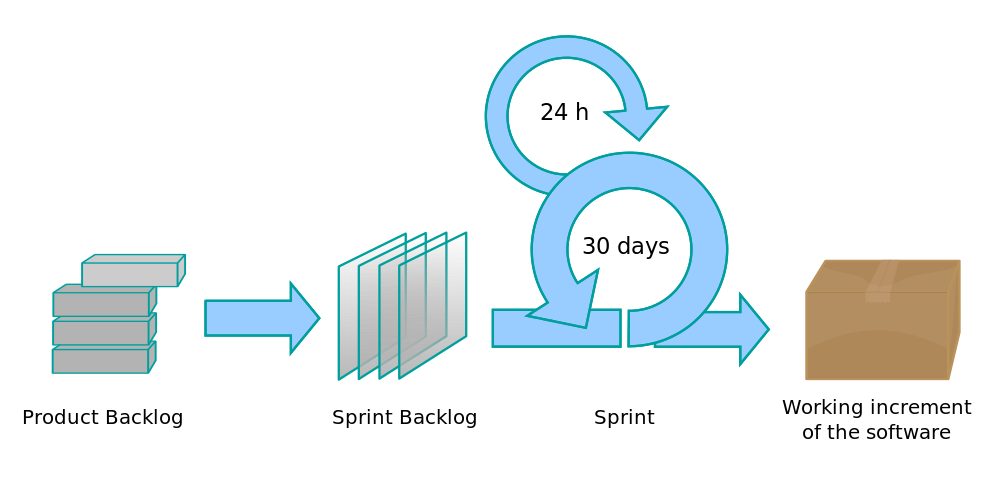
\includegraphics[scale=0.35]{graphics/scrum.png}
\caption{The Scrum Process}\label{fig:scrum_process}
\end{figure}
